\index{KIWI images!description|(}
\chapter{KIWI image description}
\label{chapter:description}
\minitoc

In order to be able to create an image with kiwi a so called
image description must be created. The image description is
represented by a directory which has to contain at least one
file named \textbf{config.xml} or alternatively \textbf{*.kiwi}.
A good start for such a description can be found in the examples
provided in /usr/share/doc/packages/kiwi/examples.

\begin{figure}[h]
\centering
\includegraphics[scale=0.5]{pictures/description.eps}
\caption{Image description directory}
\label{fig:description}
\end{figure}

The following additional information is optional for the process
of building an image but most often mandatory for the functionality
of the later operating system.

\begin{itemize}
\item \textbf{\underline{images.sh}}\\
      Optional configuration script while creating the packed image.
      This script is called at the beginning of the image creation process.
      It is designed to clean-up the image system. Affected are all the
      programs and files only needed while the unpacked image exists.

\item \textbf{\underline{config.sh}}\\
      Optional configuration script while creating the unpacked image. This
      script is called at the end of the installation but \textbf{before}
      the package scripts have run. It is designed to configure the image
      system, such as the activation or deactivation of certain services
      (insserv). The call is not made until after the switch to the image
      has been made with \textbf{chroot}.

\item \textbf{\underline{root/}}\\
      Subdirectory that contains special files, directories, and scripts for
      adapting the image environment \textbf{after} the installation of all the
      image packages. The entire directory is copied into the root of the
      image tree using \textit{cp -a}.

\item \textbf{\underline{config-yast-firstboot.xml}}\\
      Configuration file for the control of the yast2 firstboot service.
      Similar to the autoyast approach yast also provides a boot time
      service called firstboot. Unfortunately there is no GUI available
      to setup the firstboot but a good documentation in
      /usr/share/doc/packages/yast2-firstboot. Once you have 
      created such a firstboot file in your image description directory KIWI
      will process on the file and setup your image as follows:

      \begin{enumerate}
      \item KIWI enables the firstboot service
      \item While booting the image YaST is started in firstboot mode
      \item The firstboot service handles the instructions listed in the
            config-yast-firstboot.xml
      \item If the process finished successfully the environment is
            cleaned and firstboot won't be called at next reboot.
      \end{enumerate} 

\item \textbf{\underline{config-yast-autoyast.xml}}\\
      Configuration file which has been created by autoyast.
      To be able to create such an autoyast profile you should first
      call:

      \begin{Command}{8cm}
      yast2 autoyast
      \end{Command}

      Once you have saved the information from the autoyast UI as
      config-yast-autoyast.xml file in your image description directory KIWI
      will process on the file and setup your image as follows:
      \begin{enumerate}
      \item While booting the image YaST is started in autoyast mode
            automatically
      \item The autoyast description is parsed and the instructions are
            handled by YaST. In other words the \textbf{system configuration}
            is performed
      \item If the process finished successfully the environment is
            cleaned and autoyast won't be called at next reboot.
      \end{enumerate}

\item \textbf{\underline{config-cdroot.tgz}}\\
      Archive which is used for ISO images only. The data in the archive is
      uncompressed and stored in the CD/DVD root directory. This
      archive can be used, for example, to integrate a license file or
      readme information directly readable from the CD or DVD.

\item \textbf{\underline{config-cdroot.sh}}\\
      Along with the config-cdroot.tgz one can provide a script which allows
      to manipulate the extracted data.

\item \textbf{\underline{config/}}\\
      Optional Subdirectory that contains Bash scripts that are called
      after the installation of all the image packages, primarily in order
      to remove the parts of a package that are not needed for the operating
      system. The name of the Bash script must resemble the package name
      listed in the config.xml
\end{itemize}

\section{config.xml}
The mandatory image definition file is divided into different sections
which describes information like the image name and type as well as
the packages and patterns the image should consist of. The following
information explains the basic structure of the XML document. When KIWI
is called the XML structure is validated by a RelaxNG based schema.
For details on attributes and values please refer to the schema 
documentation file at /usr/share/doc/packages/ kiwi/kiwi.rng.html.

\subsection{image element}
\begin{Command}{12cm}
<image schemaversion="3.5" name="iname"\\
\hspace*{1.9cm}\textit{displayname="text"}\\
\hspace*{1.9cm}\textit{inherit="path" kiwirevision="number"}\\
\hspace*{1.9cm}\textit{id="10 digit number">}\\
\hspace*{1cm}...\\
</image>
\end{Command}

The image definition starts with an image tag and requires the
schema format at version 2.0. The attribute name specifies the
name of the image which is also used for the file names created
by KIWI. Because we don't want spaces in file names the name
attribute must not have any spaces in its name.

\begin{itemize}
\item The optional attribute displayname allows setup of the boot
      menu title for isolinux and grub. So you can have
      \textit{suse-SLED-foo} as the image name but something like
      \textit{my cool Image} as the boot display name.
\item The optional attribute inherit allows to inherit the
      packages information from another image description.
\item The optional attribute kiwirevision allows to specify
      a kiwi SVN revision number which is known to build
      a working image from this description. If the kiwi SVN
      revision is less than the specified value the
      process will exit. The currently used SVN revision can
      be queried by calling kiwi $--$version
\item The optional attribute id allows to set an identification
      number which appears as file /etc/ImageID within the
      image.
\end{itemize}

Inside the \textbf{image} section the following mandatory and optional
subelements exists. The simplest image description must define the
elements \textbf{description, preferences, repository and
packages (at least one of type=''bootstrap'')}.

\subsection{description element}
\begin{Command}{12cm}
<description type="system">\\
\hspace*{1cm}<author>an author</author>\\
\hspace*{1cm}<contact>mail</contact>\\
\hspace*{1cm}<specification>short info</specification>\\
</description>
\end{Command}

The mandatory description section contains information about
the creator of this image description. The attribute \textbf{type}
could be either of the value ''system'' which indicates this is a
system image description or at value ''boot'' for boot image
descriptions.

\subsection{profiles element}
\begin{Command}{12cm}
<profiles>\\
\hspace*{1cm}<profile name="name" description="text"/>\\
\hspace*{1cm}...\\
</profiles>
\end{Command}

The optional profiles section lets you maintain one image description
while allowing for variation of the sections packages and drivers that are
included. A separate profile element must be specified for each variation.
The profile child element, which has name and description attributes,
specifies an alias name used to mark sections as belonging to a profile,
and a short description explaining what this profile does.

To mark a set of packages/drivers as belonging to a profile, simply
annotate them with the \textbf{profiles} attribute. It is also possible
to mark sections as belonging to multiple profiles by separating the
names in the \textbf{profiles} attribute with a comma.
If a packages/drivers tag does not have a profiles attribute, it is
assumed to be present for all profiles.

\subsection{preferences element}
\begin{Command}{12cm}
<preferences \textit{profiles="name"}>\\
\hspace*{1cm}<version>1.1.2</version>\\
\hspace*{1cm}<packagemanager>smart</packagemanager>\\
\hspace*{1cm}<type image="name" ...>\\
\hspace*{2cm}<ec2config|lvmvolumes|oemconfig|pxedeploy|size|split|\\
\hspace*{2cm} vmwareconfig|xenconfig>\\
\hspace*{1cm}</type>\\
</preferences>
\end{Command}

The mandatory preferences section contains information about the supported
image type(s), the used packagemanager, the version of this image and
optional attributes. The image version must be a three-part version number of
the format: \textbf{Major}.\textbf{Minor}.\textbf{Release}. In case of
changes to the image description the following rules should apply:

\begin{itemize}
\item For smaller image modifications that do not add or remove any
      new packages, only the release number is incremented.
      The \textbf{config.xml} file remains unchanged.
\item For image changes that involve the addition or removal of packages
      the minor number is incremented and the release number is reset.
\item For image changes that change the size of the image file
      the major number is incremented.
\end{itemize}

By default kiwi use the \textbf{smart} packagemanager but it is also possible
to use the SUSE packagemanager called \textbf{zypper}. 

In general the specification of one <preferences> section is sufficient.
However, it's possible to specify multiple <preferences> sections and
distinquish between the sections via the \textbf{profiles} attribute. Data
may also be shared between different profiles. Using profiles it is possible
to, for example, configure specific preferences for OEM image generation. 
Activation of a given <preferences> during image generation is triggered by
the use of the $--$add-profile command line argument.

For each <preferences> block at least one \textbf{type} element must be
defined. It is possible to specify multiple <type> elements in any 
<preferences> block. To set a given <type> description as the default image
use the boolean attribute \textbf{primary} and set its value to \textbf{true}.
The image type to be created is determined by the value of the \textbf{image}
attribute. The following list describes the supported types and possible
values of the image attribute:

\begin{itemize}
\item \textbf{image=''cpio''}\\
      Use the cpio image type to specify the generation os a boot image
      (intrd). When generating a boot image it is possible to specify a
      specific boot profile and boot kernel using the optional
      \textbf{bootprofile=''default''} and \textbf{bootkernel=''std''}
      attributes.
      
      A boot image should group the various supported kernels into profiles. 
      If the user chooses not to us the profiles supplied by Kiwi it is
      required that one profile named \textbf{std} be created. This profile
      will be used if no other bootkernel is specified. Further it is 
      required to create a  profile named \textbf{default}. This profile is
      used when no bootprofile is specified.

      It is recommended that special configurations that omit drivers, use
      special drivers and/or special packages be specified as profiles.


      The bootprofile and bootkernel attribute are respected within the 
      definition of a system image. Us the attribute and value 
      \textbf{type="system"} of the <description> element to specify the
      creation of a system image. The values of the bootprofile and 
      bootkernel attributes are used by Kiwi when generating the boot image.
\item \textbf{image=''ec2''}\\
      Setting the image attribute value to ec2 causes the generation of
      an Amazon Machine Image (AMI) for the AWS (Amazon Web Services) 
      Elastic Compute Cloud (EC2). The AMI is an image comparable to
      a VMware or Xen guest image. It can be transferred to the AWS 
      Simple Storage Service and used within the AWS infrastructure.
      Configuration of the AMI is accomplished with the optional
      \textbf{ec2config} element, specified as a child of the <type>
      element.
\item \textbf{image=''iso''}\\
      Specify the key-value pair image=iso to generate a live system suitable
      for deployment on optical media (CD or DVD). Use the 
      \textbf{boot=''isoboot/suse-*''} attribute when generating this image
      type to select the apropriate boot image for optical media. In 
      addition the optional \textbf{flags} attribute may be set to the
      following values with the effects described below:
      \begin{itemize}
      \item \textbf{clic}: Creates a fuse based compressed read-only
            filesystem which allows write operations into a cow file.
      \item \textbf{compressed}: Compressed filesystem with squashfs and
            use a link list to mount the system read-write. An additional
            split section controls the read-write information.
      \item \textbf{dmsquash}: Creates an ext3 image file and encapsulates
            this image file within a squashfs filesystem. On boot the root 
            tree is mounted via a device mapper snapshot device to allow full 
            write access over the complete tree.
      \item \textbf{unified}: Compressed filesystem with squashfs mounted
            with an aufs based overlay mount to allow read-write access.
      \end{itemize}
      If the flags attribute is not used the filesystem will not be compressed
      and no union filesystem is used. In this case it is recommended to
      specify a \textbf{split} section as a child of this type element. The
      specification of a split block is also recommended when flags=compressed
      is used.
\item \textbf{image=''oem''}\\
      Use this type to create a virtual disk system suitable in a preload
      setting. In addition specify the attributes \textbf{filesystem}, 
      and \textbf{boot=''oemboot/suse-*''} to control the filesystem used
      for the virtual and to specify the proper boot image. Using the optional
      optional \textbf{format} attribute and setting the value to ''iso'' or 
      ''usb'' will create self installing images suitable for optical media
      or a USB stick, respectively. Booting from the media will deploy
      the OEM preload image onto the selected storage device of the
      system. It is also possible to configure the system to use logical
      volumes. Use the optional \textbf{lvm} attribute and specify the
      logical volume configuration with the \textbf{lvmvolumes} child
      element. The default volume group name is kiwiVG. Further configuration
      of the image is performed using the appropriate \textbf{*config} child
      block.
\item \textbf{image=''pxe''}\\
      Creating a network boot image is supported by Kiwi with the image=pxe
      type. When specifying the creation of a netwoork boot image use the
      \textbf{filesystem} and \textbf{boot=''netboot/suse-*''} attributes 
      to specify the filesystem of the image and the proper boot image. To
      compress the image file set the \textbf{compressed} boolean attribute
      to true. This setting will compress the image file and has no influence
      on the filesystem used within the image. The compression is often use to
      support better transfer times when the pxe image is pushed to the 
      boot server over a network connection. The pxe image layout is
      controlled by using the \textbf{pxedeploy} child element.
\item \textbf{image=''split''}\\
      The split image support allows the creation of an image as split
      files. Using this technique one can assign different filesystems and
      different read-write porperties to the different sections of the image.
      The \textbf{oem,pxe,usb and vmx} types can be created as a split system
      image. Use the \textbf{boot=''oem|netboot|usb|vmx/suse-*''} attribute
      to select the underlying type of the split image. The attributes
      \textbf{fsreadwrite}, \textbf{fsreadonly} are used to controll the
      read-write properties of the filesystem specified as the attributes
      value. Use the appropriate \textbf{*config} child block to specify
      the properties of the underlying image. For example when building a 
      OEM based split image use the \textbf{<oemconfig>} child section.
\item \textbf{image=''usb''}\\
      Use the usb value to create a USB stick image. Set the
      \textbf{filesystem} attribute to the desired supported filesystem for
      the image and use the \textbf{boot=''usbboot/suse-*''} attribute to
      select the USB boot image for the system. For a USB image you may
      also select GRUB or Syslinux as a bootloader by setting the
      optional \textbf{bootloader} attribute to grub ot syslinux,
      respectively. The USB image may also be created with LVM support.
      The same rules as indicated for the OEM image apply.
\item \textbf{image=''vmx''}\\
      Creation of a virtual disk system is enabled with the vmx value of
      the image attribute. Set the filesystem of the virtual disk with
      the \textbf{filesystem} attribute and select the appropriate boot
      image by setting \textbf{boot=''vmxboot/suse-*''}. The optional
      \textbf{format} attribute is used to specify one of the virtualization
      formats supported by qemu, such as vmdk (also the VMware format) or
      qcow2. For the virtual disk image the optional \textbf{vga} attribute
      may be used to configure the kernel framebuffer device. Acceptable
      values can be found in the Linux kernel documentation for the
      framebuffer device (Documentation/fb/vesafb.txt). Kiwi also supports
      the selection of the booloader for the virtual disk according to
      the rules indicated for the USB system. Last but not least
      the virtual disk system may also be created with a LVM based layout by
      using the \textbf{lvm} attribute. The previously indicated rules apply.
      Use the \textbf{vmwareconfig} or \textbf{xenconfig} child elements
      to specify appropriate configuration of the virtual disk system.
\item \textbf{image=''xen''}\\
      Use this type to create a Xen para-virtual guest image. The
      \textbf{filesystem} and \textbf{boot=''xenboot/suse-*''} attributes
      specify the filesystem type used and select the proper boot image,
      respectively. Use the \textbf{xenconfig} child element to specify
      configuration options of the Xen guest image.
\end{itemize}

All of the mentioned types can specify the \textbf{boot} attribute
which tells kiwi to call itself to build the requested boot image (initrd).
It is possible to tell kiwi to check for an already built boot image
which is a so called \textbf{prebuilt boot image}. To activate searching
for an appropriate prebuilt boot image the type section also provides the
attribute \textbf{checkprebuilt=''true|false''}. If specified kiwi will
search for a prebuilt boot image in a directory named
\textit{/usr/share/kiwi/image/*boot/*-prebuilt}. Example: If the boot
attribute was set to isoboot/suse-10.3 and checkprebuilt is set to true
kiwi will search the prebuilt boot image in
/usr/share/kiwi/image/isoboot/suse-10.3-prebuilt. The directory kiwi
searches for the prebuilt boot images can also be specified at the
commandline with the \textbf{$--$prebuiltbootimage} parameter.

Within the preferences section there are the following optional
attributes:

\begin{itemize}
\item \textbf{rpm-check-signatures}\\
      Specifies whether RPM should check the package signature or not
\item \textbf{rpm-excludedocs}\\
      Specifies whether RPM should skip installing package documentation
\item \textbf{rpm-force}\\
      Specifies whether RPM should be called with --force
\item \textbf{keytable}\\
      Specifies the name of the console keymap to use. The value corresponds
      to a map file in /usr/share/kbd/keymaps. The KEYTABLE variable in
      /etc/sysconfig/keyboard file is set according to the keyboard
      mapping.
\item \textbf{timezone}\\
      Specifies the time zone. Available time zones are located in the
      /usr/share/zoneinfo directory. Specify the attribute value relative to
      /usr/share/zoneinfo. For example, specify Europe/Berlin for
      /usr/share/zoneinfo/Europe/Berlin. KIWI uses this value to configure
      the timezone in /etc/localtime for the image
\item \textbf{locale}\\
      Specifies the name of the locale to use, which defines the
      contents of the RC\_LANG system environment variable in
      /etc/sysconfig/language
\item \textbf{boot-theme}\\
      Specifies the name of the gfxboot and bootsplash theme to use
\item \textbf{defaultdestination}\\
      Used if the --destdir option is not specified when calling KIWI
\item \textbf{defaultroot}\\
      Used if the option --root is not specified when calling KIWI
\item \textbf{defaultbaseroot}\\
      Used if the option --base-root is not specified when
      calling KIWI. It's possible to prepare and create an image using a
      predefined non empty root directory as base information.
      This could speedup the build process a lot if the base root path
      already contains most of the image data.
\end{itemize}

The <type> element may contain child elements to provide specific
configuration information for the given type. The following lists the 
supported child elements:

\begin{itemize}
\item \textbf{ec2config}\\
    The optional ec2config block is used to specify information relevant
    only to AWS EC2 images. The following information can be provided:

    \begin{Command}{12cm}
    <ec2config>
    \hspace*{1cm}<ec2accountnr>Your AWS account number</ec2accountnr>
    \hspace*{1cm}<ec2certfile>Path to the AWS cert-*.pem file</ec2certfile>
    \hspace*{1cm}<ec2privatekeyfile>Path to the AWS pk-*.pem file\\
       </ec2privatekeyfile>
    </ec2config>
    \end{Command}

\item \textbf{size}\\
    Specifies the size of the image with a numerical value in
    Megabytes or Gigabytes. Use the ''unit'' attribute to assign the
    unit \textbf{M} for Megabytes or \textbf{G} for Gigabytes.
    KIWI extends the image size automatically if the specified value
    is too small. If the actual size is more than 100MB larger than
    the specified size, KIWI aborts with an error
    message. KIWI does not automatically reduce the image size if
    the specified value is too large, because the extra space might
    be needed to, for example, run custom scripts. If no size is
    specified, KIWI uses the required size plus approximately
    30\% free space. The optional ''additive'' attribute can be set
    to tell kiwi to use the required size for the image plus the
    given size as additional free space. The ''additive'' attribute is
    a bool attribute and can be set to either true or false.

	\begin{Command}{12cm}
	<size unit="M">1000</size>
	\end{Command}

\item \textbf{vmwareconfig}\\
	The optional vmwareconfig section is used if the image description
	includes a packages section of type \textbf{vmware}. In this case kiwi
	is able to create the guest configuration file required to run the
	image within VMware. The guest configuration file can also be created
	by the VMware toolkit itself but with the pre-created guest configuration
	created by kiwi it is possible to provide an all in one bundle ready
	to run in VMware. The following general information can be provided to
	create the VMware (.vmx) configuration file:

	\begin{Command}{12cm}
	<vmwareconfig arch="arch" memory="MB"\\
	\hspace*{2.5cm}HWversion="number"\\
	\hspace*{2.5cm}guestOS="suse|sles"\\
	\hspace*{2.5cm}usb="true|false"/>\\
	\hspace*{1cm}<vmwarenic driver="name"\\
	\hspace*{2.5cm}interface="number" mode="mode"/>\\
	\hspace*{1cm}<vmwaredisk controller="ide|scsi"\\
	\hspace*{2.5cm}id="number"/>\\
	\hspace*{1cm}<vmwarecdrom controller="ide|scsi"\\
	\hspace*{2.5cm}id="number"/>\\
	</vmwareconfig>
	\end{Command}

	\begin{itemize}
	\item \textbf{arch}\\
      The virtualized architecture. Can be one of ix86 or x86\_64
      Bydefault ix86 is used.
	\item \textbf{memory}\\
      The mandatory memory attribute specified how much memory in MB
      should be allocated for the virtual machine
	\item \textbf{HWversion}\\
      The VMware hardware version number. By default version 3 is used
	\item \textbf{guestOS}\\
      The guestOS identifier. By default suse is used on ix86 and suse-64
      for x86\_64. At the moment only the suse and sles guestOS types
      are supported
	\item \textbf{usb}\\
      The bool value \textbf{usb} specifies whether the guest machine
      should provide a virtual USB controller or not.
	\end{itemize}

	The following information can be provided to setup the VMware virtual
	main storage device and CD/DVD drive connection.

	\begin{itemize}
	\item \textbf{controller}\\
      The mandatory controller attribute can be either ide or scsi disk
	\item \textbf{id}\\
      The mandatory id attribute specifies the disk id. If only one
      disk is set the id value should be set to 0 
	\end{itemize}

	The following information can be provided to setup the VMware virtual
	network interface

	\begin{itemize}
	\item \textbf{driver}\\
      The mandatory driver to use for the virtual network card. Possible
      values are vlance, e1000 or vmxnet. vmxnet requires the vmware tools to be
      part of the image
	\item \textbf{interface}\\
      The mandatory network interface number. If only one interface is
      set the value should be set to 0
	\item \textbf{mode}\\
      The network mode used to communicate outside the VM. In many cases
      the bridged mode is used.
	\end{itemize}

\item \textbf{xenconfig}\\
	The optional xenconfig section is used if the image description
	includes a packages section of type \textbf{xen}. In this case kiwi
	is able to create the guest configuration file required to run the
	image within Xen. According to this it's possible to provide an all
	in one bundle ready to run in Xen. The following general information
	can be provided to create the Xen (.xenconfig) configuration file:

	\begin{Command}{12cm}
	<xenconfig memory="MB"\\
	\hspace*{1cm}<xendisk device="/dev/..."/>\\
	\hspace*{1cm}<xenbridge name="eth0" mac="addr"/>\\
	</vmwareconfig>
	\end{Command}

	\begin{itemize}
	\item \textbf{memory}\\
      The mandatory memory attribute specified how much memory in MB
      should be allocated for the para virtual machine    
	\end{itemize}

	The following information can be provided to setup the Xen para virtual
	main storage device as part of a \textbf{xendisk} section

	\begin{itemize}
	\item \textbf{device}\\
      The mandatory device which should appear in the para virtual
      instance
	\end{itemize}

	The default Xen configuration uses bridging within domain 0 to allow all
	domains to appear on the network as individual hosts. In order to create
	the bridge which can be used by the Xen virtual network interface(s) the
	script ''/etc/xen/scripts/network-bridge start'' can be called to create
	a bridge as shown in the following picture:

	\begin{figure}[h]
	\centering
	\includegraphics[scale=0.5]{pictures/xenbridge.eps}
	\caption{Illustration on network-bridge and vif-bridge}
	\label{fig:architecture}
	\end{figure}

	Additional information on how to setup networking with Xen can be
	found here: \url{http://wiki.xensource.com/xenwiki/XenNetworking}
	The following information can be provided to setup the Xen network
	bridge as part of one ore more \textbf{xenbridge} section(s).

	\begin{itemize}
	\item \textbf{name}\\
      The name of the network interface which is the bridge between
      the physical device (peth) and the virtual device(s) (vif).
	\item \textbf{mac}\\
      The optional mac address value for the virtual interface inside
      the DOM(x).
	\end{itemize}

\item \textbf{pxedeploy}\\
	The optional pxedeploy section is only useful if you build the \textbf{pxe}
	image type. For this type an additional network boot infrastructure needs
	to be set up. To ease the process of setting up such a boot server kiwi
	provides a package called kiwi-pxeboot. This package sets up the basic
	pxe boot environment like kiwi expects it. The package will setup a
	directory structure in /srv/tftpboot. The result files of the kiwi
	image build process needs to be copied to that location. A detailed
	explanation of what file needs to be copied and where is provided in
	the PXE Image chapter later in this document. Among the image files itself
	it is required to provide an information how KIWI should handle the
	machine it should be install with the created image. Information like
	which image should be used or how to partition the machine needs to
	be provided in a file called config.<MAC-Address> below the directory
	/srv/tftpboot/KIWI. The reason for the pxedeploy section is to allow KIWI
	to create that file according to the information provided in the image
	description.

	\begin{Command}{14cm}
	<pxedeploy server="IP" blocksize="4096">\\
	\hspace*{1cm}<timeout>seconds</timeout>\\
	\hspace*{1cm}<commandline>kernel-options</commandline>\\
	\hspace*{1cm}<kernel>kernel-file</kernel>\\
	\hspace*{1cm}<initrd>initrd-file</initrd>\\
	\hspace*{1cm}<partitions device="/dev/sda">\\
	\hspace*{2cm}<partition type="swap" number="1" size="MB"/>\\
	\hspace*{2cm}<partition type="L" number="2" size="MB"\\
	\hspace*{4.5cm}mountpoint="/" target="true"/>\\
	\hspace*{2cm}<partition type="fd" number="3"/>\\
	\hspace*{1cm}</partitions>\\
	\hspace*{1cm}<union ro="dev" rw="dev" type="aufs|unionfs"/>\\
	\hspace*{1cm}<configuration source="/KIWI/../file" dest="/../file"\\
	\hspace*{4.5cm}arch="..."/>\\
	\hspace*{1cm}<configuration .../>\\
	</pxedeploy>
	\end{Command}

	\begin {itemize}
	\item The server and blocksize attributes specify the TFTP server which
      controls the download of image files. KIWI also supports other protocols
      than tftp but in order to do that the variables \textbf{kiwiserver} and
      \textbf{kiwiservertype} must be set as kernel parameter when the client
      boots.
	\item The optional timeout section specifies the grub timeout in seconds
      which is used when the KIWI initrd configures and installs the grub boot
      loader on the machine after the first deployment to allow standalone
      boot.
	\item The optional commandline section specifies the kernel options which
      should be passed to the kernel by the grub bootloader. the KIWI
      initrd includes this kernel options when installing the grub for
      standalone boot
	\item The optional kernel and initrd sections specifies the KIWI
      kernel and initrd files on the boot server. In case of a special boot
      method which is not supported by the distribution standard mkinitrd
      the KIWI initrd needs to stay on the system and needs to be used for
      local boot as well. So if your system image makes use of the split
      type or your pxedeploy section includes any union information the
      kernel and initrd sections must be provided.
	\item The partitions section is required if you want to install the system
      image on a disk or any other permanent storage device. Each partition is
      specified by one partition subtag which defines the type (see
      sfdisk -list-type), partition number, size, optional mountpoint, and
      optional information on if this partition is the system image
      target partition. With the KIWI netboot boot image, the first
      partition is always the swap partition, while the second partition
      is used, by default, for the system image. With the optional
      target flag, you can specify a partition other than the second
      partition to install the system image on. If size is set to ''image'',
      KIWI calculates the required size for this partition in order to
      have enough space for the later image.
	\item The optional union section is used if the system image is based
      on a read-only filesystem such as squashfs and should be mounted
      read-write by using an overlay filesystem like aufs or by a device.
      mapper setup with the dmsquash type. In this case, KIWI creates an
      additional write partition, then
      combines both partitions with the given overlay filesystem or device map.
      Currently, there are two such filesystems: unionfs and aufs
      (aufs is the preferred file system). The partition that holds the
      read-only system image must be set as the ro attribute value, and the
      partition that serves as the write partition must be set the rw
      attribute value.
	\item The optional configuration section can be used to integrate a network
      client's configuration files which are stored remotely on the server.
      The source attribute specifies the path on the server used by a
      TFTP client program to download the file, and the dest attribute
      specifies the target relative to the root (/) of the network client.
      Each file is specified by one configuration section and can be
      bound to a specific set of architectures separated by comma.
	\end{itemize}

\item \textbf{split}\\
	The optional split section is used if your image type is split or iso
	combined with the attribute compressed. The split
	section controls which files of your splitted image should be writable
	and whether they are persistantly writable or only temporarly. In case
	of an iso image all data specified can only be temporarly writable
	by design of the live system image type.

	The split section distinguishes between directory and files. The
	information of ''/etc'' would make /etc a writable directory however
	none of the files *within* /etc are affected. They remain symbolic
	links to the real files in the read-only area. The main advantage to
	putting just a directory in the read-write area is that any new
	files created there are stored on the disk instead of tmpfs. If all
	the files in /etc should also be part of the read-write area and
	according to this put a complete directory including all its files
	into the read-write area two lines are required as shown above.

	\begin{Command}{12cm}
	<split>\\
	\hspace*{1cm}<temporary>\\
	\hspace*{2cm}<!-- read/write access to: -->\\
	\hspace*{2cm}<file name="/var"/>\\
	\hspace*{2cm}<file name="/var/*"/>\\
	\hspace*{2cm}<!-- but not on this file: -->\\
	\hspace*{2cm}<except name="/etc/shadow"/>\\
	\hspace*{1cm}</temporary>\\
	\hspace*{1cm}<persistent>\\
	\hspace*{2cm}<!-- persistent read/write access to: -->\\
	\hspace*{2cm}<file name="/etc"/>\\
	\hspace*{2cm}<file name="/etc/*"/>\\
	\hspace*{2cm}<!-- but not on this file: -->\\
	\hspace*{2cm}<except name="/etc/passwd"/>\\
	\hspace*{1cm}</persistent>\\
	</split>
	\end{Command}

\item \textbf{lvmvolumes}\\
	With the optional \textbf{lvmvolumes} section you can set one or
	more top level directories into a separate volume. For example you
	want to put /usr and /var into different volumes add the following
	lvmvolumes section:

	\begin{Command}{12cm}
	<lvmvolumes>\\
	\hspace*{1cm}<volume name="usr" freespace="100M"/>\\
	\hspace*{1cm}<volume name="var" size="200M"/>\\
	</lvmvolumes>
	\end{Command}

	The optional freespace attribute let you add additional free space
	for that volume. If you don't set any freespace the volume will be
	about 80\% to 90\% full. The optional size attribute let you specify
	the absolute size for that volume. If both freespace and size are set
	size is preferred. If the given size is too small the value will be
	ignored.

\item \textbf{oemconfig}
	By default the oemboot process will create/modify a swap, /home and /
	partition. It is possible to influence the behavior by the
	oem-* elements explained below.
	KIWI uses this information to create the file
	\textbf{/config.oempartition} as part
	of the automatically created oemboot boot image. The format of the
	file is a simple key=value format and created by the KIWIConfig.sh
	function named baseSetupOEMPartition(). 

	\begin{Command}{12cm}
	<oemconfig>\\
	\hspace*{1cm}<oem-systemsize>2000</oem-systemsize>\\
	\hspace*{1cm}<oem-...\\	
	</oemconfig>
    \end{Command}

	\begin{itemize}
    \item \textbf{<oem-boot-title>text</oem-boot-title>}\\
       By default the string \textbf{OEM} will be used as the boot manager 
       menu entry when KIWI creates the grub configuration during
       deployment. The oem-boot-title element allows you to set a custom
       name for the grub menu entry. This value is represented by the
       OEM\_BOOT\_TITLE variable in config.oempartition.
	\item \textbf{<oem-home>true|false</oem-home>}\\
       Specify if a partition for the home directory should be created.
       Creation of a home partition is the default behavior. This value is 
       represented by the OEM\_WITHOUTHOME variable in config.oempartition.
	\item \textbf{<oem-kiwi-initrd>true|false</oem-kiwi-initrd>}\\
       If this element is set to true (default value is false) the oemboot 
       boot image (initrd) will \textbf{not} be replaced by the system 
       (mkinitrd) created initrd. This option is useful when the system
       is installed on removable storage such as a USB stick or a portable
       external drive. For movable devices it is potentially necessary to 
       detect the storage location during every boot. This detection
       process is part of the oemboot boot image. This value is represented
       by the OEM\_KIWI\_INITRD variable in config.oempartition.
	\item \textbf{<oem-reboot>true|false</oem-reboot>}\\
       Specify if the system is to be rebooted after the oem image has been
       deployed to the designated storage device (default value is false). 
       This value is represented by the OEM\_REBOOT variable in 
       config.oempartition
	\item \textbf{<oem-recovery>true|false</oem-recovery>}\\
      If this element is set to true (default value is false), Kiwi will
      create a recovery archivefrom the prepared root tree. The archive will 
      appear as \textit{/recovery.tar.bz2} in the image file. During 
      first boot of the image a single recovery partition will be
      created and the recovery archive will be moved to the recovery 
      partition. An additional boot menu entry is created that when selected
      restores the original root tree on the system. The
      user information on the /home partition or in the /home directory is
      not affected by the recovery process. This value is represented by 
      the OEM\_RECOVERY variable in config.oempartition.
    \item \textbf{<oem-recoveryID>partition-id</oem-recoveryID>}\\
      Specify the partition type for the recovery partition. The default 
      is to create a Linux partition (id = 83). This value is represented by 
      the OEM\_RECOVERY\_ID variable in config.oempartition. 
    \item \textbf{<oem-swap>true|false</oem-swap>}\\
       Specify if a sawp partition should be create. The creation of a swap
       partition is the default behavior. This value is represented by the
       OEM\_WITHOUTSWAP variable in config.oempartition.     
	\item \textbf{<oem-swapsize>number in MB</oem-swapsize>}\\
       Set the size of the swap partition. If a swpa partition is to be
       created and the size of the swap partition is not specified with this
       optional element, Kiwi will calculate the size of the swpar partition
       and create a swap partition equal to two times the RAM installed on
       the system at initial boot time. This value is represented by
       the OEM\_SWAPSIZE variable in config.oempartition
	\item \textbf{<oem-systemsize>number in MB</oem-systemsize>}\\
      Set the size of the root partition. This value is represented by the
      variable OEM\_SYSTEMSIZE in config.oempartition
	\end{itemize}
\end{itemize}

\subsection{users element}
\begin{Command}{12cm}
<users group="users" \textit{id="number"}>\\
\hspace*{1cm}<user pwd="..." home="dir"\\ 
\hspace*{1.5cm}name="user" \textit{id="number"}\\
\hspace*{1.5cm}\textit{pwdformat="encrypted" | "plain"}\\
\hspace*{1.5cm}\textit{realname="string"} \textit{shell="path}/>\\
\hspace*{1cm}...\\
</users>
...
\end{Command}

The optional users element specifies the users to be added to the image.
The group attribute specifies the group the users belong to. If this group
does not exist, it is created. A user element must be specified for
each group. The user child element specifies the users belonging to that
group, and the name, pwd and home attributes specifies the username,
the password, and the path to the home directory. An encrypted password can be
created using the kiwi $--$createpassword tool. If a plain text password is
given use the optional pwdformat attribute to indicate a plain text password
and Kiwi will encrypt the given password.

\subsection{drivers element}
\begin{Command}{12cm}
<drivers type="type" \textit{profiles="name"}>\\
\hspace*{1cm}<file name="filename"/>\\
\hspace*{1cm}...\\
</drivers>
\end{Command}

The optional drivers element is only useful for boot images (initrd).
As a boot image doesn't need to contain the complete kernel one can
save a lot of space if only the required drivers are part of the image.
Therefore the drivers section exists. If present only the drivers which
matches the file names or glob patterns will be included into the
boot image. The type attribute specifies one of the following driver
types:

\begin{itemize}
\item \textbf{drivers}\\
      Each file is specified relative to the
      /lib/modules/<Version>/kernel directory.
\item \textbf{netdrivers}\\
      Each file is specified relative to the
      /lib/modules/<Version>/kernel/drivers
      directory.
\item \textbf{scsidrivers}\\
      Each file is specified relative to the
      /lib/modules/<Version>/kernel/drivers
\item \textbf{usbdrivers}\\
      Each file is specified relative to the
      /lib/modules/<Version>/kernel/drivers directory.
\end{itemize}

According to the driver type the specified files are searched in
the corresponding directory. The information about the drivernames
is provided as environment variable named like the value of
the type attribute and is processed by the function
\textbf{suseStripKernel}. According to this along with a boot image
description a script called \textbf{images.sh} must exist which
calls this function in order to allow the driver information to
have any effect.

%\newpage

\subsection{repository element}
\begin{Command}{12cm}
<repository type="type"\\
\hspace*{1cm}\textit{status="replaceable"}\\
\hspace*{1cm}\textit{alias="name"}\\
\hspace*{1cm}\textit{priority="number"}>\\
\hspace*{2cm}<source path="URL"/>\\
</repository>\\
...
\end{Command}

The mandatory repository section specifies the source URL and
type used by the package manager. The type attribute specifies the
repository type which must be supported by the package manager.
At the moment KIWI supports the package managers smart and zypper
whereas smart has support for more repository types compared to
zypper. Therefore the possible values for the type attribute has
beend copied from smart. The following table shows the possible
repo types:\\ 

\begin{tabular}[h]{|p{4cm}|p{2cm}|p{2cm}|}
\hline
\textbf{type} & \textbf{smart} & \textbf{zypper} \\
\hline
apt-deb            & yes & no  \\
apt-rpm            & yes & no  \\
deb-dir            & yes & no  \\
mirrors            & yes & no  \\
red-carpet         & yes & yes \\
rpm-dir            & yes & yes \\
rpm-md             & yes & yes \\ 
slack-site         & yes & no  \\
up2date-mirrors    & yes & no  \\
urpmi              & yes & no  \\
yast2              & yes & yes \\
\hline
\end{tabular}\\

Within the repository section there are the following optional
attributes:

\begin{itemize}
\item \textbf{status=''replaceable''}\\
      This attribute makes only sense for boot image descriptions.
      It indicates that the repository is allowed to become replaced by
      the repositories defined in the system image descriptions. Because kiwi
      automatically builds the boot image if required it should create that
      image from the same repositories which are used to build the system
      image to make sure both fit together. Therefore it is required to allow
      the repository to become overwritten which is indicated by the status
      attribute.
\item \textbf{alias=''name''}\\
      Specifies an alternative name used to identify the source channel.
      If not set the source attribute value is used and builds the alias name
      by replacing each ''/'' with a ''\_''. An alias name should be set if
      the source argument doesn't really explain what this repository
      contains 
\item \textbf{priority=''number''}\\
      Specifies the repository priority assigned to all packages available in
      this repository. For \textbf{smart} the following applies: If the
      exact same package is available in more than one channel, the repository
      with the \textbf{highest} priority number is used. The value 0 means
      \textbf{no priority is set}. For \textbf{zypper} the following applies:
      If the exact same package is available in more than one channel, the
      repository with the \textbf{lowest} priority number is used. The value
      99 means \textbf{no priority is set}.
\end{itemize}

The source child element contains the path attribute, which specifies
the location (URL) of the repository. The path specification can be any
of the following, and can include the \%arch macro which is expanded
to the architecture of the image building host.

\begin{itemize}
\item \textbf{this://<path>}\\
      A relative path name, which is relative to the image
      description directory being referenced.
\item \textbf{iso://<path/to/isofile}\\
      A path to a local .iso file which is then loopback mounted
      and used as a local path based repository. Alternatively one
      can do the loop mount himself and point a standard local path
      to the mounted directory
\item \textbf{http://<url>}\\
      A http protocol based network location
\item \textbf{https://<url>}\\
      A https protocol based network location
\item \textbf{ftp://<url>}\\
      A ftp protocol based network location
\item \textbf{opensuse://<Project-Name>}\\
      A special http based network location which is created from
      the given openSUSE buildservice project name. The result is
      pointing to an rpm-md repository on the openSUSE buildservice.
      For example:\\
      path=''opensuse://openSUSE:10.3/standard''
\item \textbf{file:///local/path}\\
      A local path which should be an absolute path description.
      The file:// prefix is optional and could also be omitted.
\item \textbf{obs://\$dir1/\$dir2}\\
      A special buildservice path whereas \$dir1 and \$dir2
      represents the buildservice project location. If this type is
      used as part of a boot attribute kiwi evaluates it to
      this://images/\$dir1/\$dir2 and if used as part of a repository
      source path attribute it evaluates to this://repos/\$dir1/\$dir2
\end{itemize}

Multiple repository sections are allowed and combined by the
used package manager. By default the package manager will always use
the latest packages available.

\subsection{packages element}
\begin{Command}{12cm}
<packages type="type" \textit{profiles="name"}\\
\hspace*{2.5cm}\textit{patternType="type"}\\
\hspace*{2.5cm}\textit{patternPackageType="type"}\\
\hspace*{1cm}<package name="name" arch="arch"/>\\
\hspace*{1cm}<package name="name" replaces="name"/>\\
\hspace*{1cm}<package name="name"\\
\hspace*{2.5cm}bootinclude="true" bootdelete="true"/>\\
\hspace*{1cm}<archive name="name"\\
\hspace*{2.5cm}bootinclude="true"/>\\
\hspace*{1cm}<package .../>\\
\hspace*{1cm}<opensusePattern name="name"/>\\
\hspace*{1cm}<opensusePattern .../>\\
\hspace*{1cm}<opensuseProduct name="name"/>\\
\hspace*{1cm}<opensuseProduct .../>\\
\hspace*{1cm}<ignore name="name"/>\\
\hspace*{1cm}<ignore .../>\\
</packages>
\end{Command}

The mandatory packages element specifies the list of packages and
pattern names to be used with the image. There are five different
types of package sets or patterns, specified with the type attribute:

\begin{itemize}
\item \textbf{image}\\
      Image packages, list of packages used to finish the image
      installation. All packages which make up the image are listed here
\item \textbf{bootstrap}\\
      Bootstrap packages, list of packages used to start creating a
      new operating system root tree. Basic components which are
      required to chroot into that system, such as glibc, are listed here.

\item \textbf{delete}\\
      Delete packages, list of packages stored for later deletion.
      The package names are available in the \$delete environment
      variable of the /.profile file created by KIWI. The 
      baseGetPackagesForDeletion() function returns the contents of this
      environment variable, and can be used to delete the packages
      while ignoring requirements or dependencies. According to this
      a config.sh or images.sh script needs to be provided such as
      the following code snippet shows:
\begin{verbatim}
rpm -e --nodeps --noscripts \
   $(rpm -q `baseGetPackagesForDeletion` | grep -v "is not installed")
\end{verbatim}
\item \textbf{xen}\\
      Xen required packages, list of packages used when the image
      needs support for Xen-based virtualization.
\item \textbf{vmware}\\
      VMware required packages, list of packages used when the image
      needs support for VMware- or generic based full virtualization.
\end{itemize}

\subsubsection{Using patterns}
Using a pattern name enhances the package list with a number of
additional packages belonging to this pattern. Support for patterns
is SUSE-specific, and available with openSUSE 10.1 or later.
The optional patternType and patternPackageType attributes specify
which pattern references or packages should be used in a given pattern.
The values of these attributes are only evaluated if the KIWI pattern
solver is used. If the new (up to SUSE 11.0) satsolver pattern solver
is used these values are ignored because the satsolver can't handle
that at the moment. Allowed values for the pattern* attributes are:

\begin{itemize}
\item \textbf{onlyRequired}\\
      Incorporates only patterns and packages that are required by the
      given pattern
\item \textbf{plusSuggested}\\
      Incorporates patterns and packages that are required
      and suggested by the given pattern
\item \textbf{plusRecommended}\\
      Incorporates patterns and packages that are required and
      recommended by the given pattern.
\end{itemize}

By default, only required patterns and packages are used. The result
list of packages is solved into a clean conflict free list of packages
by the package manager. This for example means that including a suggested
package may include required and recommended packages as well according
to the dependencies. If a pattern contains unwanted packages, you can use
the ignore element to specify an ignore list, with the name attribute
containing the package name. Please note that you can't ignore a package
if it is required by a package dependency of another package in your list.
The packagemanager will automatically pull in the package even if you have
ignored it.

\subsubsection{Architecture restrictions}
To restrict a package to a specific architecture, use
the \textbf{arch} attribute to specify a comma separated list of allowed
architectures. Such a package is only installed if the build systems
architecture (uname -m) matches one of the specified values of the arch
attribute.

\subsubsection{Image type specific packages}
If a package is only required for a specific type of image
and replaces another package you can use the \textbf{replaces} attribute
to tell kiwi to install the package by replacing another one. For example
you can specify the kernel package in the type=image section as

\begin{lstlisting}[language=xml]
<package name="kernel-default" replaces="kernel-xen"/>
\end{lstlisting}

and in the type=xen section as

\begin{lstlisting}[language=xml]
<package name="kernel-xen" replaces="kernel-default"/>
\end{lstlisting}

The result is the xen kernel if you request a xen
image and the default kernel in any other case.

\subsubsection{Packages to become included into the boot image}
The optional attributes \textbf{bootinclude} and \textbf{bootdelete}
can be used to mark a package inside the system image description to
become part of the corresponding boot image (initrd). This feature
is most often used to specify bootsplash and/or graphics boot related
packages inside the system image description but they are required
to be part of the boot image as the data is used at boot time
of the image. If the bootdelete attribute is specified along with
the bootinclude attribute this means that the selected package
will be marked as a \textit{to become deleted} package and is
removed by the contents of the images.sh script of the corresponding
boot image description

\subsubsection{Data not available as packages to become included}
With the optional \textbf{archive} element it's possible to include
any kind of data into the image. The archive elements expects the
name of a tarball which must exist as part of the system image
description. kiwi then picks up the tarball and installs it into
the image. If the \textbf{bootinclude} attribute is set along with
the archive element the data will also become installed into the
boot image.



